% Section 4 -- Results and discussion (readability rewrite 28 Oct 2026). Every number is a \kn{} macro read from a results file.
\section{Results and Discussion}
\label{sec:results}

\subsection{Paddy (Common): Prices Stay at the MSP}
\label{sec:results-msp}

Table~\ref{tab:msp} describes the AGMARKNET prices~\cite{agmarknet} of the \kn{mandis} Punjab mandis that reported in all six seasons.
Together they give \kn{observed_mandi_days} mandi-days over \kn{trading_dates} trading dates, or \kn{observed_share}\% of those
possible. In 2024, \kn{msp_share_2024}\% of the reported prices were exactly the Grade-A MSP of Rs~\kn{msp_2024} per quintal, and the
mean daily standard deviation across mandis was only Rs~\kn{cross_sd_2024}. Even in the weakest season, \kn{msp_share_min_season}, the
share was \kn{msp_share_min}\%.

\begin{table}[t]
  \centering
  \caption{Paddy (Common) prices from AGMARKNET~\cite{agmarknet} in the \kn{mandis} selected Punjab mandis, September to December of each season. SD:
  standard deviation.}
  \label{tab:msp}
  \footnotesize
  % Generated by paper/template/make_numbers_tex.py. Do not edit by hand.
\begin{tabular}{@{}lrrrr@{}}
\toprule
Season & MSP Grade A & Trading & Prices equal & SD of \\
 & (Rs/q) & dates & to MSP (\%) & prices (Rs/q) \\
\midrule
2020 & 1,888 & 70 & 98.3 & 44.3 \\
2021 & 1,960 & 55 & 99.1 & 80.5 \\
2022 & 2,060 & 60 & 98.5 & 16.5 \\
2023 & 2,203 & 70 & 96.1 & 45.5 \\
2024 & 2,320 & 66 & 98.8 & 29.5 \\
2025 & 2,389 & 61 & 99.0 & 21.6 \\
\bottomrule
\end{tabular}

\end{table}

Seven forecasters were compared on the three latest seasons, 1 to 7 trading dates ahead. They were the MSP rule, which predicts the
announced Grade-A MSP, the last reported price, a seven-date average, ridge regression, a GRU, T-GCN and A3T-GCN. The MSP rule had the
lowest mean absolute error, Rs~\kn{mae_msp_mean} per quintal, followed by the last price at Rs~\kn{mae_naive_mean}. A3T-GCN was the
best learned model at Rs~\kn{mae_atgcn_mean}, slightly ahead of the GRU (Rs~\kn{mae_gru_mean}) and T-GCN (Rs~\kn{mae_tgcn_mean}).

One trading date ahead, A3T-GCN was worse than the last price on \kn{paired_atgcn_worse} of \kn{paired_dates} dates. The reason is
simple. When a mandi stays at the MSP, the last price is exactly right, and a neural network almost never predicts a change of exactly
zero. The MSP rule and the last price were close: the MSP rule was better on \kn{paired_msp_better} dates, worse on
\kn{paired_msp_worse} and equal on \kn{paired_msp_ties}. This comparison is descriptive and has no significance test. For Paddy
(Common), KisanNiti therefore uses the announced MSP as the price and trains no forecaster.

\subsection{Basmati Paddy: the Pre-Registered Forecast Comparison}
\label{sec:results-basmati}

The comparison was run once on the held-out season, after the protocol and its configuration had been frozen. Both freezes are
timestamped in the version history of the public repository. The run uses the index built from dated rows only, so the portal
inspection (Section~\ref{sec:method-data}) cannot change the primary result. Index days exist only from September to January, which
gives \kn{data_index_days_1121} index days for 1121 and \kn{data_index_days_1509} for 1509. With the ten-day rule for origins, the
held-out season yields \kn{pairs_1121_h1}, \kn{pairs_1121_h7} and \kn{pairs_1121_h14} forecast pairs at 1, 7 and 14 days for 1121, and
\kn{pairs_1509_h1}, \kn{pairs_1509_h7} and \kn{pairs_1509_h14} for 1509. For 1509 this is fewer than the 60 pairs first planned. At
28 days only \kn{pairs_1509_h28} pairs remain, below the 40 needed for a coverage claim. An exploratory power check on earlier seasons
put the smallest detectable improvement at 11 to 17\% of the naive error.

The effect of cleaning was measured before any forecast was run. Four outlier screens were tried: a past-only median absolute
deviation rule with $k=3$ and with $k=5$, a Hampel filter, and an interquartile rule. They flag between \kn{scr_madk5_flagged_pct}\%
and \kn{scr_madk3_flagged_pct}\% of the dated rows. Removing the flagged rows would change \kn{scr_madk5_changed_1121} to
\kn{scr_madk3_changed_1121} of the \kn{data_index_days_1121} index days of 1121, by up to Rs~\kn{scr_iqr15_maxchange_1121} per quintal,
and the portal inspection cannot tell which flagged rows are real errors. The rows with inferred dates look plausible. For
\kn{bd_pairs} same-day pairs of 1121 and 1509 in one market, where the second row has an inferred date, the median price ratio is
\kn{bd_ratio_inf}. For \kn{bd_control} control pairs with their own dates, one day apart, it is \kn{bd_ratio_ctl}, and the
interquartile ranges are \kn{bd_iqr_inf} and \kn{bd_iqr_ctl}. Only \kn{bd_dups} of the \kn{bd_rows} inferred rows share their key
with another row.

\begin{table}[t]
  \centering
  \caption{Held-out season 2025--26: MAE (Rs per quintal) at 1, 7 and 14 days for 1121 and 1509, and change in MAE
  against the naive forecast (\%). No change was judged better by the pre-registered rule.}
  \label{tab:forecast}
  \scriptsize
  \setlength{\tabcolsep}{3pt}
  \begin{tabular}{l|rrr|rrr}
    \toprule
    MAE & \multicolumn{3}{c|}{1121} & \multicolumn{3}{c}{1509}\\
    Method & 1 d & 7 d & 14 d & 1 d & 7 d & 14 d\\
    \midrule
    Naive & \kn{fc_1121_1_naive_mae} & \kn{fc_1121_7_naive_mae} & \kn{fc_1121_14_naive_mae} & \kn{fc_1509_1_naive_mae} & \kn{fc_1509_7_naive_mae} & \kn{fc_1509_14_naive_mae}\\
    Seasonal naive & \kn{fc_1121_1_seasonal_naive_mae} & \kn{fc_1121_7_seasonal_naive_mae} & \kn{fc_1121_14_seasonal_naive_mae} & \kn{fc_1509_1_seasonal_naive_mae} & \kn{fc_1509_7_seasonal_naive_mae} & \kn{fc_1509_14_seasonal_naive_mae}\\
    Five-day average & \kn{fc_1121_1_ma5_mae} & \kn{fc_1121_7_ma5_mae} & \kn{fc_1121_14_ma5_mae} & \kn{fc_1509_1_ma5_mae} & \kn{fc_1509_7_ma5_mae} & \kn{fc_1509_14_ma5_mae}\\
    ETS & \kn{fc_1121_1_ets_mae} & \kn{fc_1121_7_ets_mae} & \kn{fc_1121_14_ets_mae} & \kn{fc_1509_1_ets_mae} & \kn{fc_1509_7_ets_mae} & \kn{fc_1509_14_ets_mae}\\
    ARIMA & \kn{fc_1121_1_arima_mae} & \kn{fc_1121_7_arima_mae} & \kn{fc_1121_14_arima_mae} & \kn{fc_1509_1_arima_mae} & \kn{fc_1509_7_arima_mae} & \kn{fc_1509_14_arima_mae}\\
    LightGBM & \kn{fc_1121_1_lightgbm_mae} & \kn{fc_1121_7_lightgbm_mae} & \kn{fc_1121_14_lightgbm_mae} & \kn{fc_1509_1_lightgbm_mae} & \kn{fc_1509_7_lightgbm_mae} & \kn{fc_1509_14_lightgbm_mae}\\
    GRU & \kn{fc_1121_1_gru_mae} & \kn{fc_1121_7_gru_mae} & \kn{fc_1121_14_gru_mae} & \kn{fc_1509_1_gru_mae} & \kn{fc_1509_7_gru_mae} & \kn{fc_1509_14_gru_mae}\\
    Chronos-2 & \kn{fc_1121_1_chronos2_mae} & \kn{fc_1121_7_chronos2_mae} & \kn{fc_1121_14_chronos2_mae} & \kn{fc_1509_1_chronos2_mae} & \kn{fc_1509_7_chronos2_mae} & \kn{fc_1509_14_chronos2_mae}\\
    \midrule
    Change vs naive (\%) & & & & & &\\
    Seasonal naive & \kn{inf_1121_1_seasonal_naive_rel} & \kn{inf_1121_7_seasonal_naive_rel} & \kn{inf_1121_14_seasonal_naive_rel} & \kn{inf_1509_1_seasonal_naive_rel} & \kn{inf_1509_7_seasonal_naive_rel} & \kn{inf_1509_14_seasonal_naive_rel}\\
    Five-day average & \kn{inf_1121_1_ma5_rel} & \kn{inf_1121_7_ma5_rel} & \kn{inf_1121_14_ma5_rel} & \kn{inf_1509_1_ma5_rel} & \kn{inf_1509_7_ma5_rel} & \kn{inf_1509_14_ma5_rel}\\
    ETS & \kn{inf_1121_1_ets_rel} & \kn{inf_1121_7_ets_rel} & \kn{inf_1121_14_ets_rel} & \kn{inf_1509_1_ets_rel} & \kn{inf_1509_7_ets_rel} & \kn{inf_1509_14_ets_rel}\\
    ARIMA & \kn{inf_1121_1_arima_rel} & \kn{inf_1121_7_arima_rel} & \kn{inf_1121_14_arima_rel} & \kn{inf_1509_1_arima_rel} & \kn{inf_1509_7_arima_rel} & \kn{inf_1509_14_arima_rel}\\
    LightGBM & \kn{inf_1121_1_lightgbm_rel} & \kn{inf_1121_7_lightgbm_rel} & \kn{inf_1121_14_lightgbm_rel} & \kn{inf_1509_1_lightgbm_rel} & \kn{inf_1509_7_lightgbm_rel} & \kn{inf_1509_14_lightgbm_rel}\\
    GRU & \kn{inf_1121_1_gru_rel} & \kn{inf_1121_7_gru_rel} & \kn{inf_1121_14_gru_rel} & \kn{inf_1509_1_gru_rel} & \kn{inf_1509_7_gru_rel} & \kn{inf_1509_14_gru_rel}\\
    Chronos-2 & \kn{inf_1121_1_chronos2_rel} & \kn{inf_1121_7_chronos2_rel} & \kn{inf_1121_14_chronos2_rel} & \kn{inf_1509_1_chronos2_rel} & \kn{inf_1509_7_chronos2_rel} & \kn{inf_1509_14_chronos2_rel}\\
    \bottomrule
  \end{tabular}
\end{table}

Table~\ref{tab:forecast} gives the held-out MAE of each method and its change against the naive forecast. Under the pre-registered
rule, \kn{inf_better} of the \kn{inf_total} comparisons found a method better than the naive forecast. The largest raw improvement came from the GRU one
day ahead for 1121, a change in MAE of \kn{inf_1121_1_gru_rel}\% (Rs~\kn{fc_1121_1_gru_mae} against Rs~\kn{fc_1121_1_naive_mae}). Its
bootstrap interval excluded zero, but its Holm-adjusted $p$ was \kn{inf_1121_1_gru_p}, so it does not count as better. Where a method
did differ significantly from the naive forecast, it was worse. The seasonal naive forecast was significantly worse in
\kn{inf_worse_sig} comparisons; for 1509 one day ahead its MAE changed by \kn{inf_1509_1_seasonal_naive_rel}\% (adjusted $p$
\kn{inf_1509_1_seasonal_naive_p}).

This does not mean that all methods are equal. In \kn{inf_excl_gain} of the \kn{inf_total} comparisons, the interval rules out an
improvement as large as the smallest detectable gain. The other \kn{inf_inconclusive} are inconclusive rather than negative. They
include all \kn{inf_h1_1121_inconclusive} non-seasonal methods one day ahead for 1121, where improvements of up to about a quarter are
still consistent with the data (median interval width \kn{inf_width_median} points). For prices that move this little, the naive
forecast is hard to beat. The system therefore uses it, together with ranges, and states that the baseline is sufficient.

The protocol also declared \kn{sens_done} variants of the index: with inferred dates included, with sub-yards merged, and with at
least 2 or 4 mandis a day. Repeating the comparisons on all of them, with the configuration already chosen, gave the same picture.
Across the \kn{sens_comparisons} comparisons, \kn{sens_better} found a better method, and apart from the seasonal naive forecast no
method differed significantly (\kn{sens_other_significant} cases).

The secondary and descriptive horizons are reported without tests. At 28 days, the GRU and LightGBM had a lower MAE than the naive
forecast for 1121 (Rs~\kn{fc_1121_28_gru_mae} for the GRU against Rs~\kn{fc_1121_28_naive_mae}). Both models use the day of the season
as an input, so this is a hypothesis to test in later seasons, not a finding. The partly observed season 2026--27 was run separately
and is reported descriptively. It gives only \kn{pro_1121_1_pairs} pairs one day ahead for 1121 and \kn{pro_1509_1_pairs} for 1509,
falling to \kn{pro_1509_14_pairs} at 14 days, which is too few for a test. For 1509 the naive forecast had the lowest MAE at 7 and 14
days (Rs~\kn{pro_1509_7_naive_mae} and Rs~\kn{pro_1509_14_naive_mae}).

The 80\% and 95\% ranges were checked at the three primary horizons. The models' own ranges, from ETS, ARIMA, LightGBM quantiles and
Chronos-2, were well calibrated in \kn{rng_native_calibrated} of \kn{rng_native_total} cases, too wide in \kn{rng_native_over} and too
narrow in \kn{rng_native_under}. The split-conformal ranges did worse. They were calibrated on the residuals of a single, more volatile
validation season, and they were well calibrated in only \kn{rng_conf_calibrated} of
\kn{rng_conf_total} cases and too wide in \kn{rng_conf_over}. One season is not enough to calibrate a range.

\subsection{Allocation: Fair Plans Against Simple Rules}
\label{sec:results-alloc}

Before any comparison, the solver was checked against brute-force enumeration, which shares only the input types and the exact
objective with it. On \kn{alloc_oracle_instances} random small instances, three solver back ends were run with two leximin methods:
HiGHS~\cite{highs}, the Solving Constraint Integer Programs (SCIP) solver and the CP-SAT solver of Google OR-Tools. In
\kn{alloc_oracle_agree} of \kn{alloc_oracle_cases} runs the solver reached exactly the objective found by enumeration.

The method was then compared with simpler rules on \kn{allpol_plans} weekly plans. The plans come from ten draws of a synthetic FPO
with 300 members whose lots become ready over six weeks. They are scored with real 2025 AGMARKNET prices~\cite{agmarknet} of Paddy
(Common) and real mandi coordinates, with road distance taken as 1.3 times the straight-line distance. Every plan is re-checked by the
independent validator. Table~\ref{tab:alloc} compares seven policies: the nearest mandi; each farmer's independent best choice; a plan
that maximizes only total net return (utilitarian); a plan that maximizes only the smallest share; a greedy water-filling heuristic;
the KisanNiti hierarchy; and, as a bound, the same hierarchy run with actual instead of forecast prices.

\begin{table}[t]
  \centering
  \caption{Selling policies on \kn{allpol_plans} synthetic plans at real 2025 prices. Valid: plans accepted by the independent validator (a plan is invalid if it exceeds a mandi's daily limit). Net: mean net return (Rs per quintal). Min.\ share: smallest share of a lot sold, averaged over plans. Fairness price: net return given up against the utilitarian plan.}
  \label{tab:alloc}
  \scriptsize
  \begin{tabular}{lrrrrrr}
    \toprule
    Policy & Valid (\%) & Net & Min.\ share (\%) & Gini & Fairness price & Solve (s)\\
    \midrule
    Nearest mandi & \kn{allpol_p1_nearest_all_valid_pct} & \kn{allpol_p1_nearest_net_rs_per_q} & \kn{allpol_p1_nearest_min_fulfilment_pct} & \kn{allpol_p1_nearest_gini_fulfilment} & \kn{allpol_p1_nearest_price_of_fairness_rs_per_q} & \kn{allpol_p1_nearest_seconds_mean}\\
    Independent best & \kn{allpol_p2_independent_all_valid_pct} & \kn{allpol_p2_independent_net_rs_per_q} & \kn{allpol_p2_independent_min_fulfilment_pct} & \kn{allpol_p2_independent_gini_fulfilment} & -- & \kn{allpol_p2_independent_seconds_mean}\\
    Utilitarian & \kn{allpol_utilitarian_all_valid_pct} & \kn{allpol_utilitarian_net_rs_per_q} & \kn{allpol_utilitarian_min_fulfilment_pct} & \kn{allpol_utilitarian_gini_fulfilment} & \kn{allpol_utilitarian_price_of_fairness_rs_per_q} & \kn{allpol_utilitarian_seconds_mean}\\
    Max-min only & \kn{allpol_maxmin_all_valid_pct} & \kn{allpol_maxmin_net_rs_per_q} & \kn{allpol_maxmin_min_fulfilment_pct} & \kn{allpol_maxmin_gini_fulfilment} & \kn{allpol_maxmin_price_of_fairness_rs_per_q} & \kn{allpol_maxmin_seconds_mean}\\
    Greedy & \kn{allpol_greedy_all_valid_pct} & \kn{allpol_greedy_net_rs_per_q} & \kn{allpol_greedy_min_fulfilment_pct} & \kn{allpol_greedy_gini_fulfilment} & \kn{allpol_greedy_price_of_fairness_rs_per_q} & \kn{allpol_greedy_seconds_mean}\\
    KisanNiti & \kn{allpol_kisaniti_all_valid_pct} & \kn{allpol_kisaniti_net_rs_per_q} & \kn{allpol_kisaniti_min_fulfilment_pct} & \kn{allpol_kisaniti_gini_fulfilment} & \kn{allpol_kisaniti_price_of_fairness_rs_per_q} & \kn{allpol_kisaniti_seconds_mean}\\
    Actual-price bound & \kn{allpol_perfect_foresight_all_valid_pct} & \kn{allpol_perfect_foresight_net_rs_per_q} & \kn{allpol_perfect_foresight_min_fulfilment_pct} & \kn{allpol_perfect_foresight_gini_fulfilment} & \kn{allpol_perfect_foresight_price_of_fairness_rs_per_q} & \kn{allpol_perfect_foresight_seconds_mean}\\
    \bottomrule
  \end{tabular}
\end{table}

When each farmer chose independently, a mandi's daily limit was broken in \kn{allpol_p2_independent_runs_with_violation_pct}\% of the
plans, so none of these plans was valid. The nearest-mandi rule respects the limits, but its least-served farmer sold only
\kn{allpol_p1_nearest_min_fulfilment_pct}\% of their lot. The utilitarian plan did no better
(\kn{allpol_utilitarian_min_fulfilment_pct}\%), because maximizing the total ignores who is left out. The KisanNiti hierarchy raised the
smallest share to \kn{allpol_kisaniti_min_fulfilment_pct}\%, the most that the mandi limits allow, with a Gini coefficient of
\kn{allpol_kisaniti_gini_fulfilment}. This fairness cost Rs~\kn{allpol_kisaniti_price_of_fairness_rs_per_q} per quintal against the
utilitarian plan. The greedy rule reached the same smallest share but gave up Rs~\kn{allpol_greedy_price_of_fairness_rs_per_q} per
quintal.

Using actual instead of forecast prices changed nothing. This was expected, because prices of Paddy (Common) hardly differ between
mandis (Section~\ref{sec:results-msp}); distance, limits and fairness decide the plan. Of the \kn{allpol_exact_solves} exact solves,
\kn{allpol_exact_proven} were proven optimal. Three weighted-sum alternatives hit the 300-second limit without proving optimality in a
six-plan pilot, so they are left out of Table~\ref{tab:alloc}. Because the FPO is synthetic, these results describe how the method
behaves, not a gain for any real farmer.

The transport rate and the daily limit are assumed values, so the comparison was repeated for \kn{alloc_sens_settings} combinations of
three rates (Rs 1, 2 and 4 per quintal-km) and three limits (200, 300 and 500 quintals per mandi-day). Figure~\ref{fig:sensitivity}
shows the results. The KisanNiti plan was valid in every setting. The smallest share it secures rises with the limit, from
\kn{alloc_sens_kis_min_fulfilment_min}\% to \kn{alloc_sens_kis_min_fulfilment_max}\%, because no plan can sell more than the mandis can
take, and it does not depend on the rate. Compared with the nearest-mandi rule, the KisanNiti plan gains Rs~\kn{alloc_sens_kis_gain_vs_p1_min}
to Rs~\kn{alloc_sens_kis_gain_vs_p1_max} per quintal, and its price of fairness ranges from Rs~\kn{alloc_sens_kis_pof_min} to
Rs~\kn{alloc_sens_kis_pof_max}. The price of fairness grows with the transport rate. The greedy heuristic gave up more net return than
the exact plan in \kn{alloc_sens_greedy_costlier} of \kn{alloc_sens_settings} settings. The nearest-mandi rule left at least one farmer
with no sale whenever the limit was 300 quintals or less.

\begin{figure}[t]
  \centering
  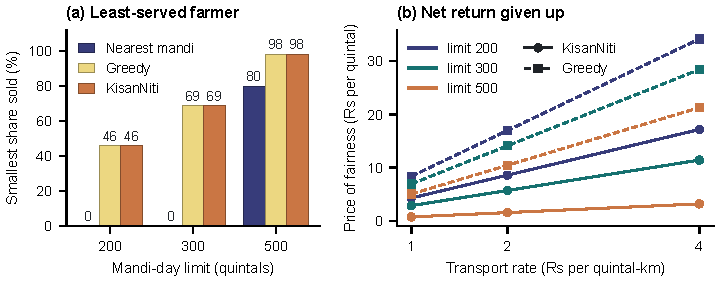
\includegraphics[width=\textwidth]{fig_allocation_sensitivity.pdf}
  \caption{Allocation under nine settings of transport rate and mandi-day limit, \kn{allpol_plans} synthetic plans each. (a) Smallest
  share of a lot sold; it is the same for every transport rate. (b) Net return given up against the utilitarian plan (price of
  fairness) by the exact KisanNiti plan (solid) and the greedy heuristic (dashed).}
  \label{fig:sensitivity}
\end{figure}

Solve times were measured on random instances with 10 to 1,000 farmers, 5 to 25 mandis and 3 to 14 days, with a 60-second limit and
three seeds each. HiGHS and SCIP proved optimality on every instance with up to 100 farmers; at 100 farmers their median times were
\kn{alloc_scaling_highs_100_median_s} and \kn{alloc_scaling_scip_100_median_s} seconds. At 300 and 1,000 farmers they reached the time
limit with a feasible plan. CP-SAT proved optimality only at 10 farmers, because its integer scaling grows too large beyond that. The
greedy heuristic needed under \kn{alloc_scaling_greedy_1000_median_s} seconds even at 1,000 farmers, and every plan a solver returned
was valid. The 300-member synthetic FPO above was solved exactly in \kn{allpol_kisaniti_seconds_mean} seconds on average (maximum
\kn{allpol_kisaniti_seconds_max}). Instance structure clearly matters, so larger or less regular FPOs should be solved with a time limit
and the greedy plan as a fallback.

\subsection{Checking the Manager's Edits}
\label{sec:results-edits}

A manager's edit should be accepted exactly when it keeps the plan valid. To test this, a second checker was written directly from
the rules: choices must be admissible, lines must not repeat, quantities must come in whole increments, no lot may be over-allocated
(or left over when the whole lot must be sold), and no mandi may exceed its limit. The edits were made at random on
\kn{val_instances} solved instances and ranged from harmless changes to a single broken rule; \kn{val_valid} were valid and
\kn{val_invalid} invalid. The second checker gave the same verdict as the independent validator on \kn{val_agree} of the
\kn{val_edits} edits.

% Section 4.4 -- storage rule on simulated scenarios (readability rewrite 28 Oct 2026; details in paper/sections/_supplement_storage.tex).
\subsection{Storage Rule on Simulated Scenarios}
\label{sec:results-storage}

The rule was evaluated on \kn{stor_scenarios} simulated scenarios built from the monthly climate normals of the India Meteorological
Department station at Patiala~\cite{imd2022}. Each scenario was run with \kn{stor_seeds} noise seeds and with sensor biases of
$\pm2$\,\%RH. Without bias, the rule agreed with the intended category in \kn{stor_s3_demo_agree}--\kn{stor_s2_demo_agree}\,\% of known
hours in the four in-grain scenarios, and it changed category at most \kn{stor_demo_flips_max} times a week. A rule that uses only the
latest reading changed category \kn{stor_instant_flips_min}--\kn{stor_instant_flips_max} times a week, and shed-air humidity was a poor
stand-in for the grain. The 24-hour median has two costs. It is slower, reporting HIGH about \kn{stor_s2_demo_highdelay}\,h late, and it
returns UNKNOWN more often. A sensor error of $\pm2$\,\%RH mattered as much as the choice of rule and caused up to
\kn{stor_demo_falsehigh_biasplus_max}\,\% false HIGH hours, so every sensor needs a salt calibration before its readings are used. These
tests measure how far noise and shortcuts move the rule away from its definition. The definition itself rests on the storage
literature~\cite{gwinner1996}\cite{delucia1994}.


\subsection{The Built System}
\label{sec:results-system}

The system has \kn{sys_tests_total} automated tests. Among other things, they cover parallel approvals on PostgreSQL, isolation
between FPOs, append-only records and the exact text of every message. The system also has \kn{sys_slices} versioned contracts with
\kn{sys_examples_valid} valid and \kn{sys_examples_invalid} invalid examples.

A single command runs \kn{sys_chain_steps} steps on two new fictional FPOs through the same interface that the website uses. The steps
cover data, stock, a simulated sensor, the plan, an edit, approval, messages, the manager's hand-over to WhatsApp, sales, release, a
ledger audit and isolation. Each step is checked against an independent recomputation, and the run stops at the first deviation. It
passed all \kn{sys_chain_passed} steps in about \kn{sys_chain_seconds} seconds. Faults planted on purpose were each detected: a corrupted
ledger entry, rounding down, a wrong weighted price and a message missing its last character. All farmers, lots and sales in this run
are fictional, and no message went to a real farmer. The English, Punjabi and Hindi message texts were checked by independent
reviewers. Figure~\ref{fig:app} shows three screens of the manager app after this run: the approved revision of a plan, the approved
plan as a Punjabi message to one farmer, and the planned against the actual sale.

\begin{figure}[t]
  \centering
  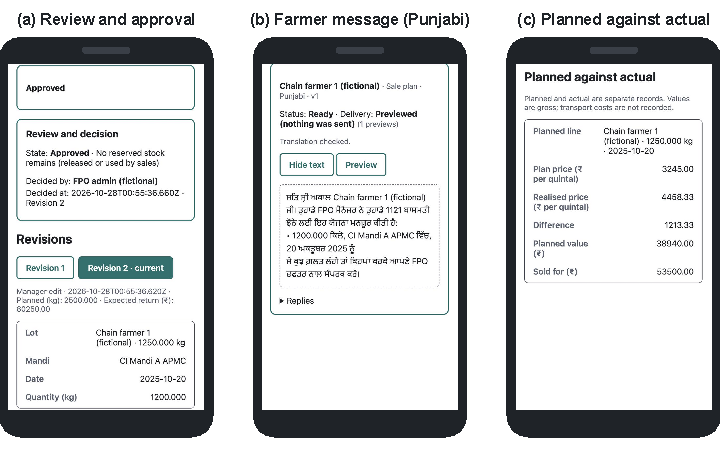
\includegraphics[width=\textwidth]{fig_app_screens.pdf}
  \caption{Manager app on a phone after the end-to-end run on a fictional FPO. (a) The manager's edit is stored as revision 2 and
  approved. (b) The approved plan written in Punjabi for one farmer, built from a reviewed template. (c) The sale recorded from the
  J-form, compared with the plan.}
  \label{fig:app}
\end{figure}
